\chapter{Copulas and Its Applications}

Copulae (or couplas) are an interesting mathematical tool to represent correlations between probability distributions. They can be used to represent complex dependencies in multivariate risk models, when more basic tools such as multivariate Gaussian distributions are inappropriate. Another commonly used application is sampling from correlated random variables.

In this Chapter the copula concept is reviewed and some example application are shown. However before going into the copulas we need to learn how to transform a distribution into another using the \emph{probability integral transform}. 

%The concept will be described in this chapter together with practical applications in computing default probabilities in multinamed contracts like CDOs and Basket Default Swaps.

\section{Distribution Transformation}\label{distribution-transformation}

Distribution transformation is a very useful tool which will be
extensively used with the copula concept that we discuss in the next
Section. The technique we are going to outline transforms every random
variables regardless its distribution into uniform and vice versa and is called
\emph{probability integral transform} or (percentile-to-percentile
transform).

Computationally, this method involves computing the quantile function (see Section~\ref{quantile-function}) of
a distribution, in other words, computing the cumulative
distribution function (CDF) of a distribution (which maps a number in
the domain to a probability between 0 and 1) and then inverting that
function. We won't go into the details but we will just show few
examples of how this can be done in \(\tt{python}\).

Imagine we want to 
The transformation takes uniform samples of a number \(u\) between 0 and
1, interpreted as a probability, and then returns the largest number
\(x\) from the domain of the distribution \(\mathbb{P}(X)\) such that
\(\mathbb{P}(-\infty <X<x)\le u\). For example, imagine that
\(\mathbb{P}(X)\) is the standard normal distribution with mean zero and
standard deviation one. Table~\ref{tab:transformation} below shows samples taken from the
uniform distribution and their representation on the standard normal
distribution.

\begin{table}[h]
  \centering
  \begin{tabular}{|c|c|}
    \hline
    \(\mathbf{u}\) & \(\mathbf{F^{-1}(u)}\) \\
    \hline
    0.5 & 0 \\
        \hline
        .975 & 1.95996 \\
            \hline
            .995 & 2.5758 \\
                \hline
                .999999 & 4.75342 \\
                    \hline
                    \(1-2^{-52}\) & 8.12589 \\
                        \hline
  \end{tabular}
  \caption{Comparison of values of the uniform distribution and the corresponding Gaussian quantiles.}
\label{tab:transformation}
\end{table}

Now let's see how this can be done with \texttt{python}, the first step is to sample
uniformly distributed values between 0 and 1, in the left plot of Fig.~\ref{fig:uniform_and_gauss} the resulting distribution is shown:

\begin{tcolorbox}[breakable, size=fbox, boxrule=1pt, pad at break*=1mm,colback=cellbackground, colframe=cellborder]
\begin{Verbatim}[commandchars=\\\{\}]
\PY{k+kn}{from} \PY{n+nn}{scipy} \PY{k}{import} \PY{n}{stats}
\PY{n}{x} \PY{o}{=} \PY{n}{stats}\PY{o}{.}\PY{n}{uniform}\PY{p}{(}\PY{l+m+mi}{0}\PY{p}{,} \PY{l+m+mi}{1}\PY{p}{)}\PY{o}{.}\PY{n}{rvs}\PY{p}{(}\PY{l+m+mi}{10000}\PY{p}{)}
\end{Verbatim}
\end{tcolorbox}

    Next we want to transform these samples so that instead of uniform they
are normally distributed. As we have seen the transform that does this
is the inverse of the cumulative density function (CDF) of the normal
distribution the \((\tt{ppf(x))}\). In the right plot of Fig.~\ref{fig:uniform_and_gauss} the Gaussian transform is shown

\begin{figure}[h]
  \centering
  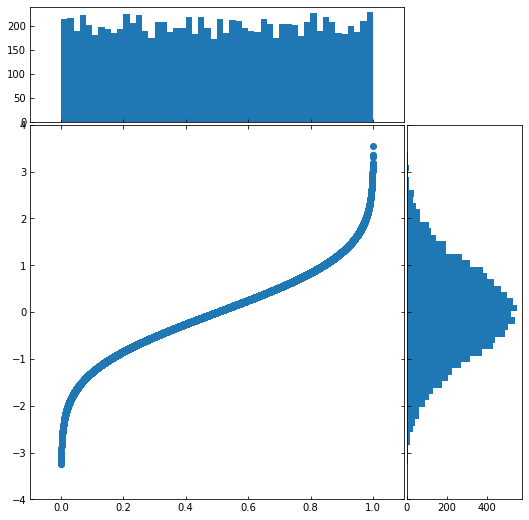
\includegraphics[width=0.45\textwidth]{copula_files/copula_5_0.png}\qquad
  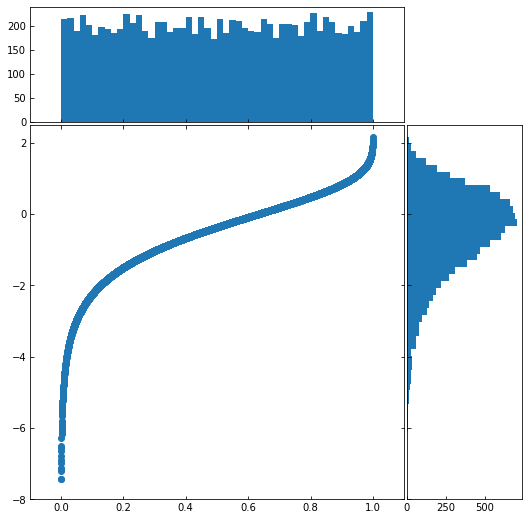
\includegraphics[width=0.45\textwidth]{copula_files/copula_7_0.png}
  \caption{On the left the generated uniform distribution, on the right its Gaussian transform.}
  \label{fig:uniform_and_gauss}
\end{figure}

\begin{tcolorbox}[breakable, size=fbox, boxrule=1pt, pad at break*=1mm,colback=cellbackground, colframe=cellborder]
\begin{Verbatim}[commandchars=\\\{\}]
\PY{n}{norm} \PY{o}{=} \PY{n}{stats}\PY{o}{.}\PY{n}{distributions}\PY{o}{.}\PY{n}{norm}\PY{p}{(}\PY{p}{)} 
\PY{n}{x\PYZus{}trans} \PY{o}{=} \PY{n}{norm}\PY{o}{.}\PY{n}{ppf}\PY{p}{(}\PY{n}{x}\PY{p}{)}
\end{Verbatim}
\end{tcolorbox}

    If we plot them togeter in a 2D plot we can get a sense of what is
going on using the inverse CDF transformation.
The inverse CDF stretches the outer regions of the uniform to yield a
normal distribution. The transformation is shown in Fig.~\ref{fig:uniform_to_gauss}. 
    
\begin{figure}[htb]
  \centering
  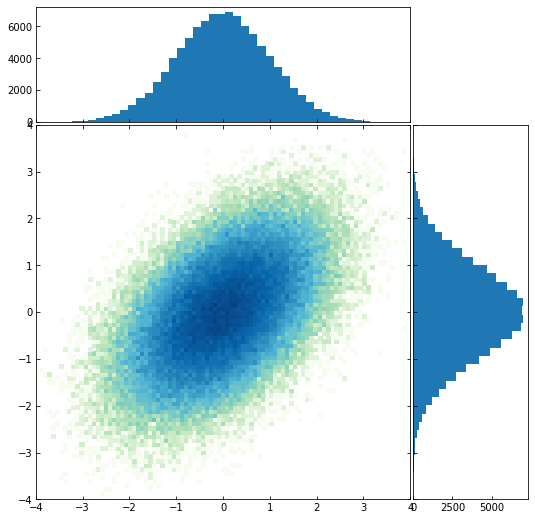
\includegraphics[width=0.5\textwidth]{copula_files/copula_9_0.png}
  \caption{2D plot showing the transformation that maps our initial uniform distribution to the resulting Gaussian.}
  \label{fig:uniform_to_gauss}
\end{figure}
    
The nice thing of the technique is that it can be
done for any arbitrary (univariate) probability distributions, like for
example \href{https://en.wikipedia.org/wiki/Student\%27s\_t-distribution}{t-Student}
or \href{https://en.wikipedia.org/wiki/Gumbel_distribution}{Gumbel}.
A similar transformation from Uniform to t-Student distribution is shown in Fig.~\ref{fig:uniform_to_tstudent}.

\begin{figure}[htb]
  \centering
  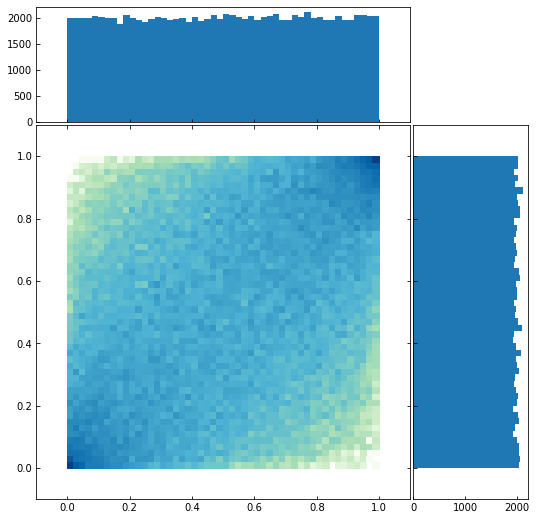
\includegraphics[width=0.5\textwidth]{copula_files/copula_11_0.png}
  \caption{2D plot showing the transformation that maps a uniform distribution to a t-Student.}
  \label{fig:uniform_to_tstudent}
\end{figure}

    Clearly to do the opposite transformation from an arbitray distribution
to the uniform(0, 1) we can just apply the inverse of the inverse CDF,
the CDF itself\ldots{}


\section{Copula}\label{copula}

In probability theory a \emph{copula} \(C(U_1, U_2, \ldots, U_n, \rho)\)
is a multivariate (multidimensional) cumulative distribution function
for which the marginal probability distribution (the probability
distribution of each dimension) of each variable is uniform on the
interval \([0, 1]\) (\(U_i \approx\)Uniform(0,1)).
\(\rho\) represent the correlation between each variable.

\emph{Sklar's theorem} states that any multivariate joint distribution
can be written in terms of univariate marginal distribution functions
and a copula which describes the dependence structure between the
variables.

Copulas are used to describe the dependence between random variables and
have been used widely in quantitative finance to model and minimize tail
risk and portfolio-optimization applications. Copulas are popular since
they allow one to easily model and estimate the distribution of random
vectors by estimating marginals and copulae separately.

Despite the obscure and daunting definition the conceptof copula is
quite simple so let's try to clarify it a bit with a practical example.
Later we will see what role copulas played in the 2008 financial crisis.

\subsection{Example Problem Case}\label{example-problem-case}

Imagine we measure two variables that are non-normally distributed and
correlated. For example, we look at various rivers and for every river
we look at the maximum water level of that river over a certain
time-period. In addition, we also count how many months each river
caused flooding.

For the probability distribution of the maximum level of the river we
know that maximums are Gumbel distributed, while the number of flooding
can be modelled according to a
\href{https://en.wikipedia.org/wiki/Beta_distribution}{\emph{Beta}}
distribution.

Clearly it is pretty reasonable to assume that the maximum level and the
number of floodings is going to be correlated, however we don't know how
we could model that correlated probability distribution. Above we only
specified the distributions for individual variables, irrespective of
the other one (i.e.~the marginals), in reality we are dealing with a
joint distribution of both of these together.

And here is where copulas come to our rescue.

Copulas essentially allow to decompose a joint probability distribution
into their marginals (which by definition have no correlation) and a
function which couples (hence the name) them together and thus allows us
to specify the correlation separately. The copula is that coupling
function.

\subsection{Adding Correlation with Gaussian
Copulas}\label{adding-correlation-with-gaussian-copulas}

How does this help us with our problem of creating a custom joint
probability distriution ?

We are actually almost done already, we saw before how to convert
anything uniformly distributed to an arbitrary probability distribution.
So that means we need to generate uniformly distributed data with the
correlation we want and then transform the marginals into the desired
distributions.

How do we do that ?

\begin{itemize}
\tightlist
\item
  simulate from a multivariarte Gaussian with the specific corrrelation
  structure;
\item
  transform so that the marginals are uniform
\item
  finally transform the uniform marginals to whatever we like.
\end{itemize}

So let's sample from a multivariate normal (2D) with a 0.5 correlation, see Fig.~ \ref{fig:multivariate_with_correlation}.

\begin{tcolorbox}[breakable, size=fbox, boxrule=1pt, pad at break*=1mm,colback=cellbackground, colframe=cellborder]
\begin{Verbatim}[commandchars=\\\{\}]
\PY{n}{mvnorm} \PY{o}{=} \PY{n}{stats}\PY{o}{.}\PY{n}{multivariate\PYZus{}normal}\PY{p}{(}\PY{n}{mean}\PY{o}{=}\PY{p}{[}\PY{l+m+mi}{0}\PY{p}{,} \PY{l+m+mi}{0}\PY{p}{]} \PY{p}{,} \PY{n}{cov}\PY{o}{=}\PY{p}{[}\PY{p}{[}\PY{l+m+mi}{1}\PY{p}{,} \PY{l+m+mf}{0.5}\PY{p}{]}\PY{p}{,}
                                                      \PY{p}{[}\PY{l+m+mf}{0.5}\PY{p}{,} \PY{l+m+mi}{1}\PY{p}{]}\PY{p}{]}\PY{p}{)}
\PY{n}{x} \PY{o}{=} \PY{n}{mvnorm}\PY{o}{.}\PY{n}{rvs}\PY{p}{(}\PY{l+m+mi}{100000}\PY{p}{)}
\end{Verbatim}
\end{tcolorbox}

\begin{figure}[htb]
  \centering
  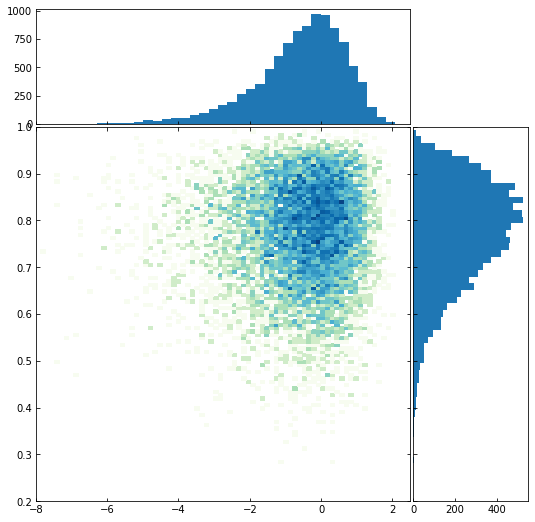
\includegraphics[width=0.5\textwidth]{copula_files/copula_15_0.png}
  \caption{2D multivariate normal distribution with a correlation factor of 0.5.}
  \label{fig:multivariate_with_correlation}
    \end{figure}
    
    Now use what we have just seen to \emph{uniformify} the marginals using
the \(\tt{cdf}\) function of the normal distribution (\(x\) is a 2D
vector, but in the code we can treat it as a vector, \(\tt{cdf}\) will
be applied separately on each component):

\begin{tcolorbox}[breakable, size=fbox, boxrule=1pt, pad at break*=1mm,colback=cellbackground, colframe=cellborder]
\begin{Verbatim}[commandchars=\\\{\}]
\PY{n}{norm} \PY{o}{=} \PY{n}{stats}\PY{o}{.}\PY{n}{norm}\PY{p}{(}\PY{p}{)}
\PY{n}{x\PYZus{}unif} \PY{o}{=} \PY{n}{norm}\PY{o}{.}\PY{n}{cdf}\PY{p}{(}\PY{n}{x}\PY{p}{)}
\end{Verbatim}
\end{tcolorbox}

The plots shown in Fo.~\ref{fig:copula} are usually how copulas are visualized.

    \begin{figure}
    \centering
    %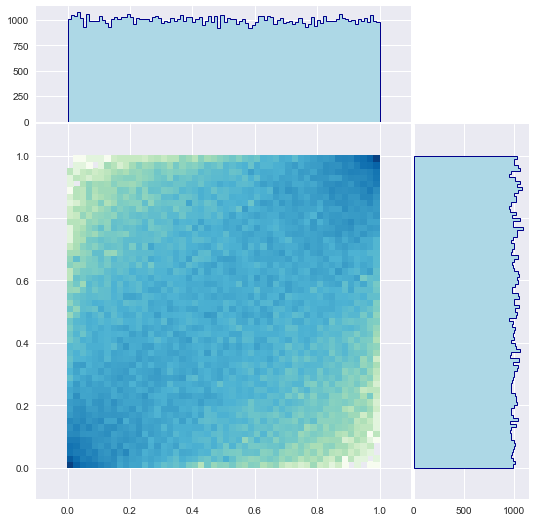
\includegraphics[width=0.45\textwidth]{copula_files/copula_17_0.png}
    \quad
    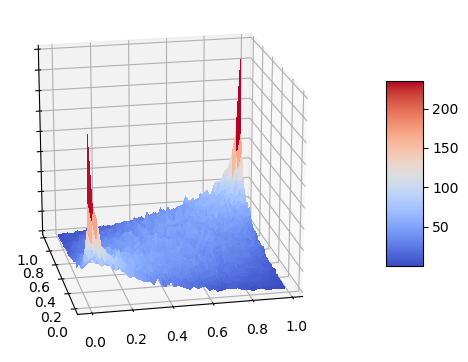
\includegraphics[width=0.5\textwidth]{copula_3d.png}
    \caption{Graphical representations of the copula, 2D on the left, 3D on the right.}
    \label{fig:copula}
    \end{figure}

Finally we can just transform the marginals again from uniform to what we want
(i.e.~Gumbel and Beta in our river example):

\begin{tcolorbox}[breakable, size=fbox, boxrule=1pt, pad at break*=1mm,colback=cellbackground, colframe=cellborder]
\begin{Verbatim}[commandchars=\\\{\}]
\PY{n}{m1} \PY{o}{=} \PY{n}{stats}\PY{o}{.}\PY{n}{gumbel\PYZus{}l}\PY{p}{(}\PY{p}{)}
\PY{n}{m2} \PY{o}{=} \PY{n}{stats}\PY{o}{.}\PY{n}{beta}\PY{p}{(}\PY{n}{a}\PY{o}{=}\PY{l+m+mi}{10}\PY{p}{,} \PY{n}{b}\PY{o}{=}\PY{l+m+mi}{3}\PY{p}{)}
\PY{n}{m1} \PY{o}{=} \PY{n}{stats}\PY{o}{.}\PY{n}{gumbel\PYZus{}l}\PY{p}{(}\PY{p}{)}
\PY{n}{m2} \PY{o}{=} \PY{n}{stats}\PY{o}{.}\PY{n}{beta}\PY{p}{(}\PY{n}{a}\PY{o}{=}\PY{l+m+mi}{10}\PY{p}{,} \PY{n}{b}\PY{o}{=}\PY{l+m+mi}{3}\PY{p}{)}
\end{Verbatim}
\end{tcolorbox}

Figure~\ref{fig:gumbel_beta_with_corr} shows the two marginal and the joint distribution.

\begin{figure}[htb]
  \centering
%  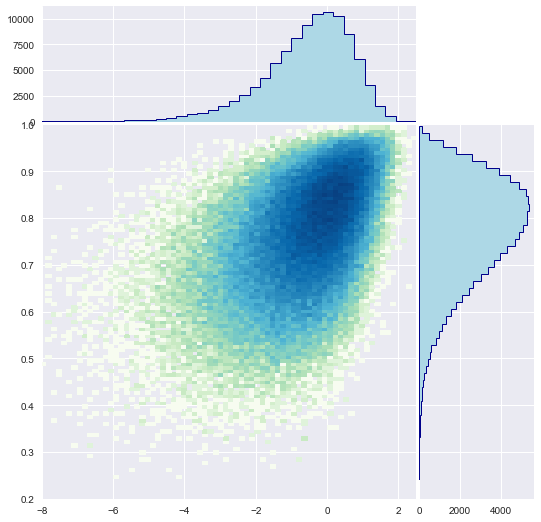
\includegraphics[width=0.5\textwidth]{copula_files/copula_19_0.png}
  \caption{Marginalized Gumbel and Beta distributions and their joint with Gaussian copula correlation.}
  \label{fig:gumbel_beta_with_corr}
\end{figure}
    
    To see that it is actually working as expected we should now compare the joint
    distribution with and without correlation. Compare Fig.~\ref{fig:gumbel_beta_with_corr} and~\ref{fig:gumbel_beta_without_corr} to see the
    difference.

\begin{tcolorbox}[breakable, size=fbox, boxrule=1pt, pad at break*=1mm,colback=cellbackground, colframe=cellborder]
\begin{Verbatim}[commandchars=\\\{\}]
\PY{c+c1}{\PYZsh{} sample from Gumbel}
\PY{n}{x1} \PY{o}{=} \PY{n}{m1}\PY{o}{.}\PY{n}{rvs}\PY{p}{(}\PY{l+m+mi}{10000}\PY{p}{)}
\PY{c+c1}{\PYZsh{} sample from Beta}
\PY{n}{x2} \PY{o}{=} \PY{n}{m2}\PY{o}{.}\PY{n}{rvs}\PY{p}{(}\PY{l+m+mi}{10000}\PY{p}{)}
\end{Verbatim}
\end{tcolorbox}

\begin{figure}[htb]
  \centering
%  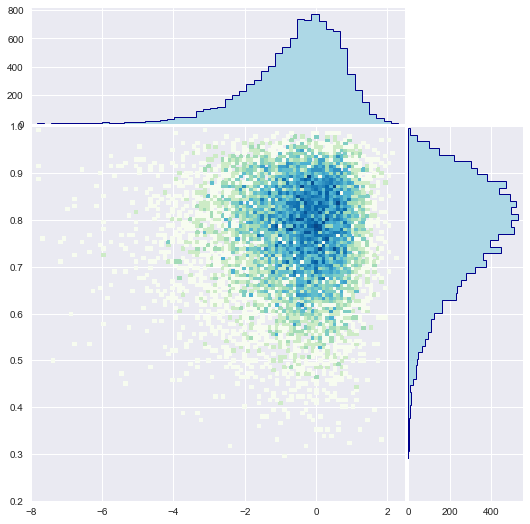
\includegraphics[width=0.5\textwidth]{copula_files/copula_21_0.png}
  \caption{Marginalized Gumbel and Beta distributions and their joint without correlation.}
  \label{fig:gumbel_beta_without_corr}
\end{figure}
    
    Using the uniform distribution as a common base for our transformations
we can easily introduce correlations and flexibly construct complex
probability distributions. Clearly this is directly extendeable to
higher dimensional distributions as well.

\subsubsection{Generate Correlated Distributions}\label{generate-correlated-distributions}

If we need to generate numbers from correlated distribution we can
follow the same steps as before:

\begin{itemize}
\tightlist
\item
  generate a random vector \(\mathbf{x}=(x_1, x_2,\ldots)\) from the
  original multivariate distribution;
\item
  determine the single \(U_i(x_i)\) by applying \(\tt{cdf}\) to each
  \(x_i\);
\item
  transform again each \(U_i(x_i)\) to the desired marginal
  distributions using \(\tt{ppf}\);
\item
  each component of the vector \(\mathbf{x}\) could be converted to a set
  of random numbers drawn from the desired distributions, with the
  appropriate correlation.
\end{itemize}

A practical application concerns the probability of default. 
Imagine there are three companies ($A$, $B$ and $C$) which have a
cumulative probability of defaulting within the next two years of 10\%.
Let's try to compute the probabilities to have the three of them all
defaulting within the next three years in the case where the default
probabilities are independent and in the, similar unrealistic, case where
they are perfectly correlated.

In the first case (independent probabilities), the
odds to get three defaults within two years will be the product
of the single probabilities, hence:

\[\mathbb{P}_{\mathrm{uncorr}} = 10\% \cdot 10\% \cdot 10\% = 0.1 \%\]

We can verify this in \(\tt{python}\) by applying the method outlined
above: generate a random sample from an uncorrelated multivariate normal
distribution, then transform each sample (\([x_A, x_B, x_C]\)) into the
uniform distribution with the \(\tt{norm.cdf}\) function (i.e. we
convert the samples into probabilities) and then count how many times the
three of them are lower than 10\%.

\begin{tcolorbox}[breakable, size=fbox, boxrule=1pt, pad at break*=1mm,colback=cellbackground, colframe=cellborder]
\begin{Verbatim}[commandchars=\\\{\}]
\PY{k+kn}{from} \PY{n+nn}{scipy}\PY{n+nn}{.}\PY{n+nn}{stats} \PY{k}{import} \PY{n}{multivariate\PYZus{}normal}\PY{p}{,} \PY{n}{uniform}\PY{p}{,} \PY{n}{norm}
\PY{k+kn}{import} \PY{n+nn}{numpy}
	
\PY{n}{numpy}\PY{o}{.}\PY{n}{random}\PY{o}{.}\PY{n}{seed}\PY{p}{(}\PY{l+m+mi}{10}\PY{p}{)}
\PY{n}{trials} \PY{o}{=}\PY{l+m+mi}{10000}
\PY{n}{mvnorm\PYZus{}no\PYZus{}corr} \PY{o}{=} \PY{n}{multivariate\PYZus{}normal}\PY{p}{(}\PY{n}{mean}\PY{o}{=}\PY{p}{[}\PY{l+m+mi}{0}\PY{p}{,} \PY{l+m+mi}{0}\PY{p}{,} \PY{l+m+mi}{0}\PY{p}{]}\PY{p}{,} \PY{n}{cov}\PY{o}{=}\PY{p}{[}\PY{p}{[}\PY{l+m+mi}{1}\PY{p}{,} \PY{l+m+mi}{0}\PY{p}{,} \PY{l+m+mi}{0}\PY{p}{]}\PY{p}{,}
                                                          \PY{p}{[}\PY{l+m+mi}{0}\PY{p}{,} \PY{l+m+mi}{1}\PY{p}{,} \PY{l+m+mi}{0}\PY{p}{]}\PY{p}{,}
                                                          \PY{p}{[}\PY{l+m+mi}{0}\PY{p}{,} \PY{l+m+mi}{0}\PY{p}{,} \PY{l+m+mi}{1}\PY{p}{]}\PY{p}{]}\PY{p}{)}
	
\PY{n}{defaults} \PY{o}{=} \PY{l+m+mi}{0}
\PY{n}{x} \PY{o}{=} \PY{n}{mvnorm\PYZus{}no\PYZus{}corr}\PY{o}{.}\PY{n}{rvs}\PY{p}{(}\PY{n}{trials}\PY{p}{)}
\PY{n}{x\PYZus{}trans} \PY{o}{=} \PY{n}{norm}\PY{o}{.}\PY{n}{cdf}\PY{p}{(}\PY{n}{x}\PY{p}{)}
\PY{k}{for} \PY{n}{i} \PY{o+ow}{in} \PY{n+nb}{range}\PY{p}{(}\PY{n+nb}{len}\PY{p}{(}\PY{n}{x\PYZus{}trans}\PY{p}{)}\PY{p}{)}\PY{p}{:}
    \PY{k}{if} \PY{n}{x\PYZus{}trans}\PY{p}{[}\PY{n}{i}\PY{p}{]}\PY{p}{[}\PY{l+m+mi}{0}\PY{p}{]} \PY{o}{\PYZlt{}} \PY{l+m+mf}{0.1} \PY{o+ow}{and} \PY{n}{x\PYZus{}trans}\PY{p}{[}\PY{n}{i}\PY{p}{]}\PY{p}{[}\PY{l+m+mi}{1}\PY{p}{]} \PY{o}{\PYZlt{}} \PY{l+m+mf}{0.1} \PY{o+ow}{and} \PY{n}{x\PYZus{}trans}\PY{p}{[}\PY{n}{i}\PY{p}{]}\PY{p}{[}\PY{l+m+mi}{2}\PY{p}{]} \PY{o}{\PYZlt{}} \PY{l+m+mf}{0.1}\PY{p}{:}
	\PY{n}{defaults} \PY{o}{+}\PY{o}{=} \PY{l+m+mi}{1}
	
\PY{n+nb}{print} \PY{p}{(}\PY{l+s+s2}{\PYZdq{}}\PY{l+s+s2}{Defaults w/o correlation: }\PY{l+s+si}{\PYZob{}:.2f\PYZcb{}}\PY{l+s+s2}{\PYZpc{}}\PY{l+s+s2}{\PYZdq{}}\PY{o}{.}\PY{n}{format}\PY{p}{(}\PY{n}{defaults}\PY{o}{/}\PY{n}{trials}\PY{o}{*}\PY{l+m+mi}{100}\PY{p}{)}\PY{p}{)}

Defaults w/o correlation: 0.10\%
\end{Verbatim}
\end{tcolorbox}
The result is 0.1\% as expected.

If we repeat the same Monte Carlo experiment with perfectly correlated
default probabilities we have

\begin{tcolorbox}[breakable, size=fbox, boxrule=1pt, pad at break*=1mm,colback=cellbackground, colframe=cellborder]
\begin{Verbatim}[commandchars=\\\{\}]
\PY{n}{mvnorm\PYZus{}corr} \PY{o}{=} \PY{n}{multivariate\PYZus{}normal}\PY{p}{(}\PY{n}{mean}\PY{o}{=}\PY{p}{[}\PY{l+m+mi}{0}\PY{p}{,}\PY{l+m+mi}{0}\PY{p}{,}\PY{l+m+mi}{0}\PY{p}{]}\PY{p}{,} \PY{n}{cov}\PY{o}{=}\PY{p}{[}\PY{p}{[}\PY{l+m+mi}{1}\PY{p}{,} \PY{l+m+mf}{0.999999}\PY{p}{,} \PY{l+m+mf}{0.999999}\PY{p}{]}\PY{p}{,}
                                                     \PY{p}{[}\PY{l+m+mf}{0.999999}\PY{p}{,} \PY{l+m+mi}{1}\PY{p}{,} \PY{l+m+mf}{0.999999}\PY{p}{]}\PY{p}{,}
                                                     \PY{p}{[}\PY{l+m+mf}{0.999999}\PY{p}{,} \PY{l+m+mf}{0.999999}\PY{p}{,} \PY{l+m+mi}{1}\PY{p}{]}\PY{p}{]}\PY{p}{)}
\PY{n}{defaults} \PY{o}{=} \PY{l+m+mi}{0}
\PY{n}{x} \PY{o}{=} \PY{n}{mvnorm\PYZus{}corr}\PY{o}{.}\PY{n}{rvs}\PY{p}{(}\PY{n}{trials}\PY{p}{)}
\PY{n}{x\PYZus{}trans} \PY{o}{=} \PY{n}{norm}\PY{o}{.}\PY{n}{cdf}\PY{p}{(}\PY{n}{x}\PY{p}{)}
\PY{k}{for} \PY{n}{i} \PY{o+ow}{in} \PY{n+nb}{range}\PY{p}{(}\PY{n+nb}{len}\PY{p}{(}\PY{n}{x\PYZus{}trans}\PY{p}{)}\PY{p}{)}\PY{p}{:}
    \PY{k}{if} \PY{n}{x\PYZus{}trans}\PY{p}{[}\PY{n}{i}\PY{p}{]}\PY{p}{[}\PY{l+m+mi}{0}\PY{p}{]} \PY{o}{\PYZlt{}} \PY{l+m+mf}{0.1} \PY{o+ow}{and} \PY{n}{x\PYZus{}trans}\PY{p}{[}\PY{n}{i}\PY{p}{]}\PY{p}{[}\PY{l+m+mi}{1}\PY{p}{]} \PY{o}{\PYZlt{}} \PY{l+m+mf}{0.1} \PY{o+ow}{and} \PY{n}{x\PYZus{}trans}\PY{p}{[}\PY{n}{i}\PY{p}{]}\PY{p}{[}\PY{l+m+mi}{2}\PY{p}{]} \PY{o}{\PYZlt{}} \PY{l+m+mf}{0.1}\PY{p}{:}
        \PY{n}{defaults} \PY{o}{+}\PY{o}{=} \PY{l+m+mi}{1}

\PY{n+nb}{print} \PY{p}{(}\PY{l+s+s2}{\PYZdq{}}\PY{l+s+s2}{Defaults w/ correlation: }\PY{l+s+si}{\PYZob{}:.2f\PYZcb{}}\PY{l+s+s2}{\PYZpc{}}\PY{l+s+s2}{\PYZdq{}}\PY{o}{.}\PY{n}{format}\PY{p}{(}\PY{n}{defaults}\PY{o}{/}\PY{n}{trials}\PY{o}{*}\PY{l+m+mi}{100}\PY{p}{)}\PY{p}{)}

Defaults w/ correlation: 9.89\%
\end{Verbatim}
\end{tcolorbox}
In this case the result is 10\%, like we had only one single company,
indeed being perfectly correlated either there is no default or three
"simultaneous" defaults with 10\% probability.

\section{Complex Correlation Structures and the Financial
Crisis}\label{complex-correlation-structures-and-the-financial-crisis}

In the example above we have used the multivariate normal which gave
rise to the Gaussian copula.However, we can use other and more complex
copulas as well. For example we might want to assume the correlation is
non-symmetruc which is useful in quant finance where correlations become
very strong during market crashes and returns very negative.

Infact, Gaussian copulas are said to have played a key role in the 2008
financial crisis as tail-correlations were severely underestimated.
Consider a set of mortgages in CDOs (a particular kind of contract that
we are going to see) they are clearly correlated, if one mortgage fails,
the likelihood that another failing is increased. In the early 2000s,
the banks only knew how to model the marginals of the default rates. An
(in)famous paper by Li then suggested to use copulas to model the
correlations between those marginals. Rating agencies relied on thid
model so heaviy, severely underestimating risk and giving false
ratings\ldots{}

If you are interested in the argument read
\href{http://samueldwatts.com/wp-content/uploads/2016/08/Watts-Gaussian-Copula_Financial_Crisis.pdf}{this paper}
for an excellent description of Gaussian copulas and the Financial
Crisis which argues that different copula choices would not have made a
difference but instead the assumed correlation was way too low.
